\section{Background}

\begin{frame}{What is an Evolutionary Transition in Individuality?}

\begin{itemize}[<+->]
\item a new, more complex replicating entity is derived from the combination of cooperating replicating entities that have irrevocably entwined their long-term fates \cite{west2015major}
\item e.g., aerobe endosymbiosis $\rightarrow$ Eukaryotes w/ mitochondria \cite{sagan1967origin}
\item key to the complexification and diversification of biological life \cite{smith1997major}
\item highlighted w.r.t. open-ended evolution \cite{ray1996evolving, banzhaf2016defining}
\end{itemize}

\end{frame}

\begin{frame}{What is a Fraternal Transition in Individuality?}

key distinction: closely-related entities (kin) unite

\pause

\vspace{6ex}

\begin{figure}
\begin{columns}
\begin{column}{0.27\textwidth}
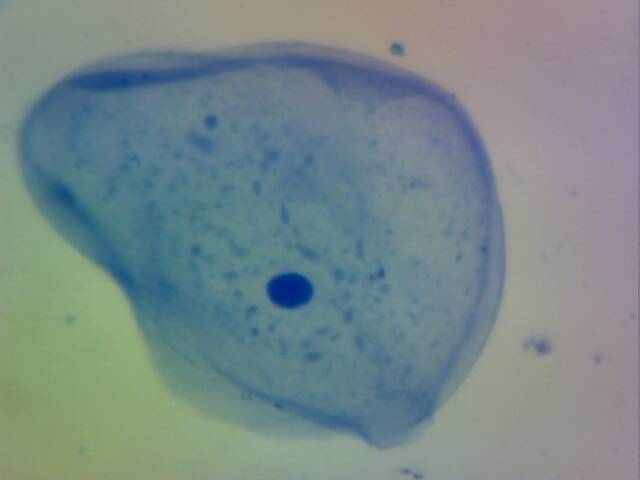
\includegraphics[width=\textwidth]{cheek_cell}
\end{column}
\begin{column}{0.07\textwidth}

\includegraphics[width=\textwidth]{arrow}
\end{column}
\begin{column}{0.27\textwidth}
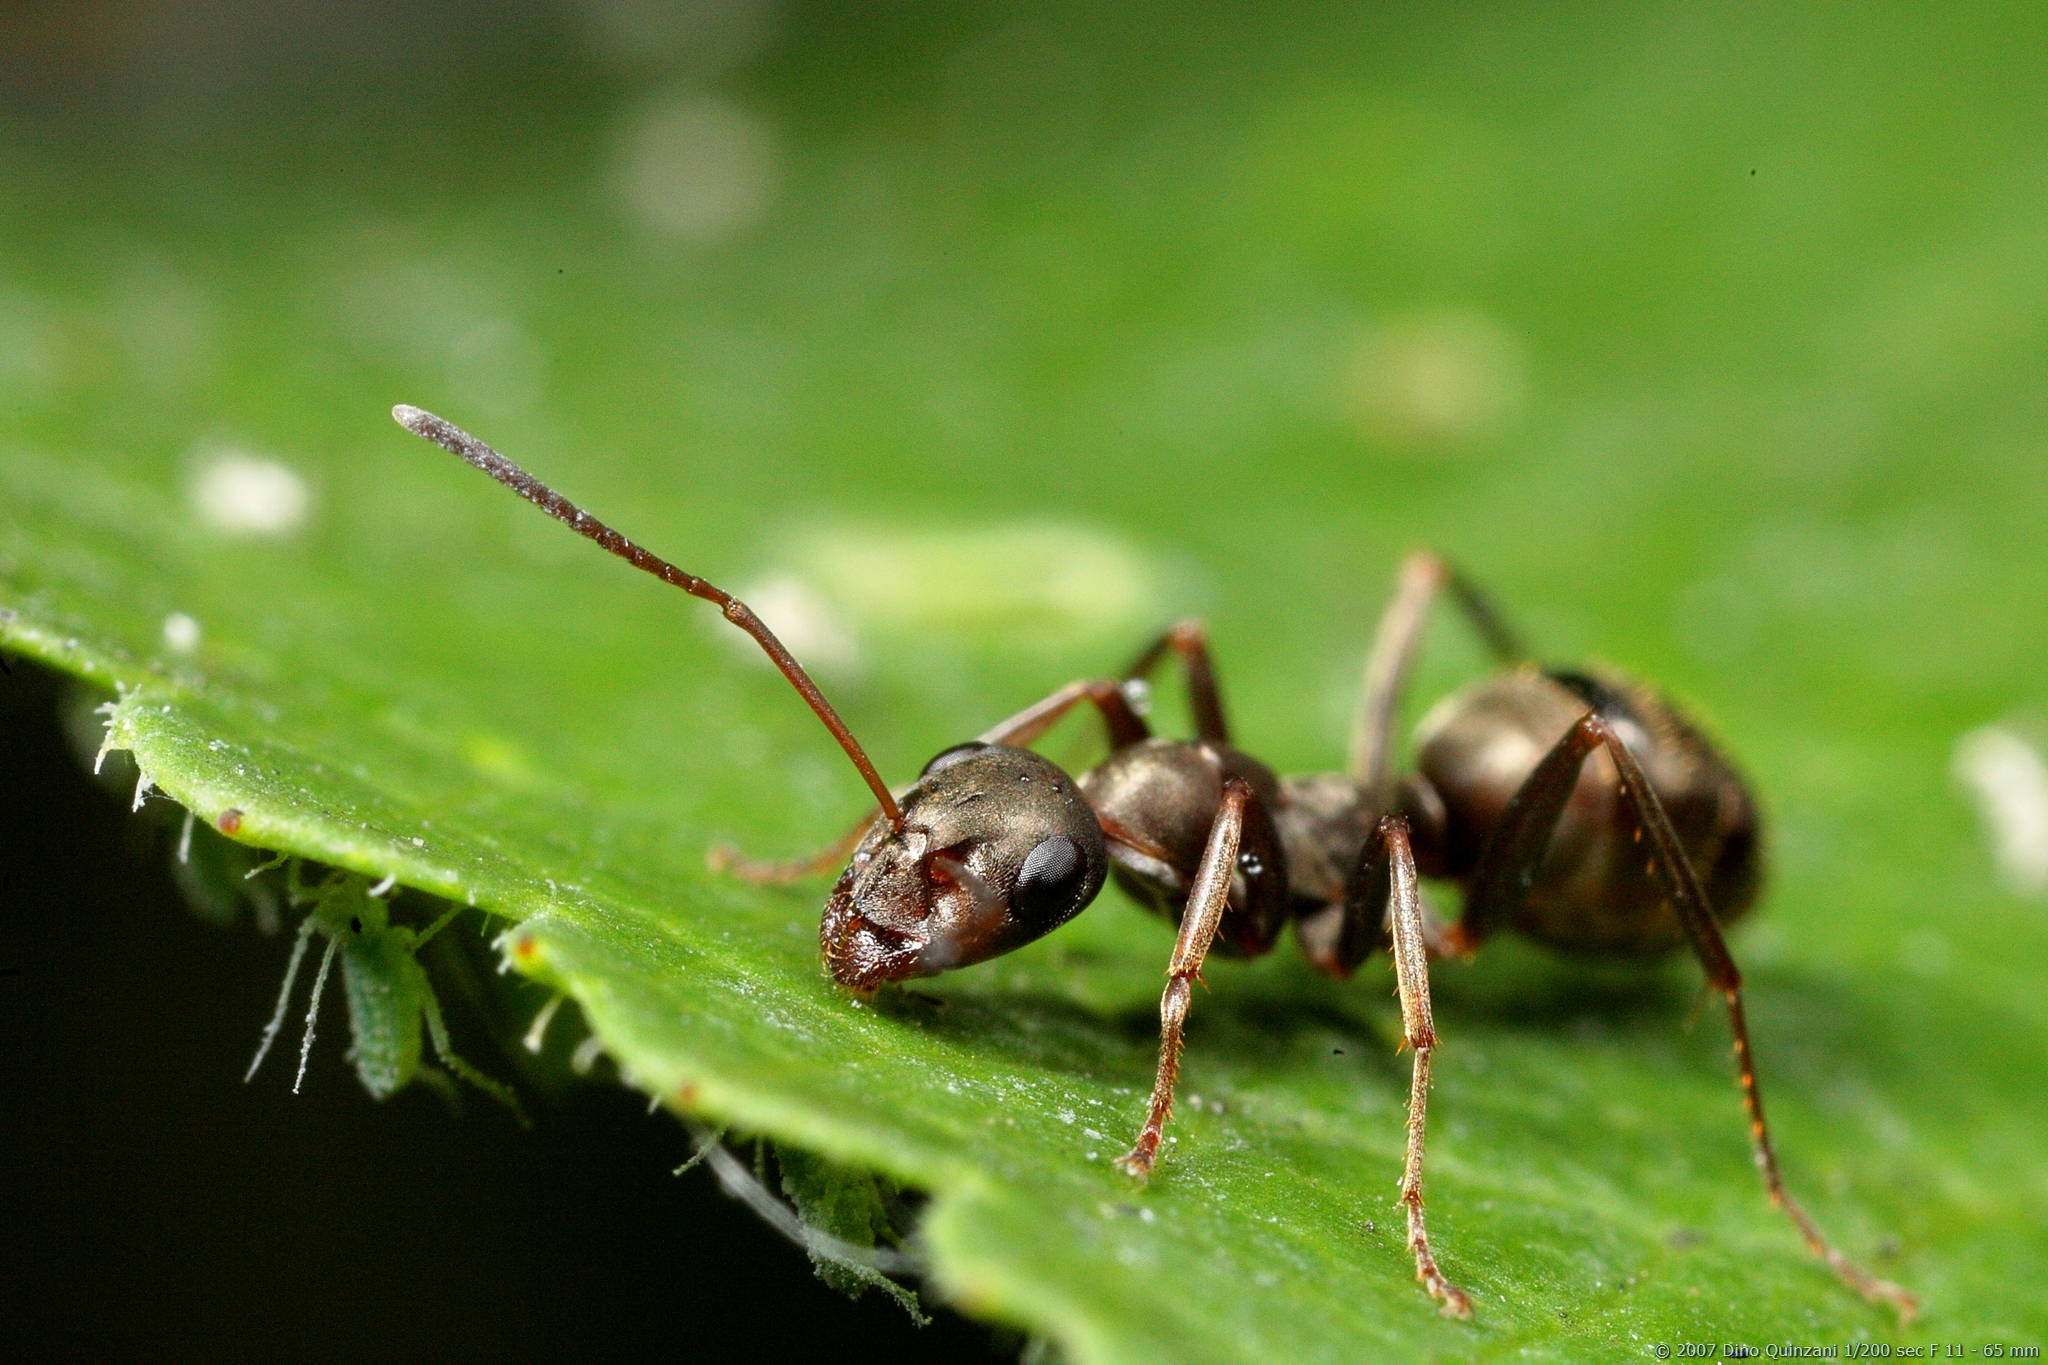
\includegraphics[width=\textwidth]{ant}
\end{column}
\begin{column}{0.07\textwidth}

\includegraphics[width=\textwidth]{arrow}
\end{column}
\begin{column}{0.27\textwidth}
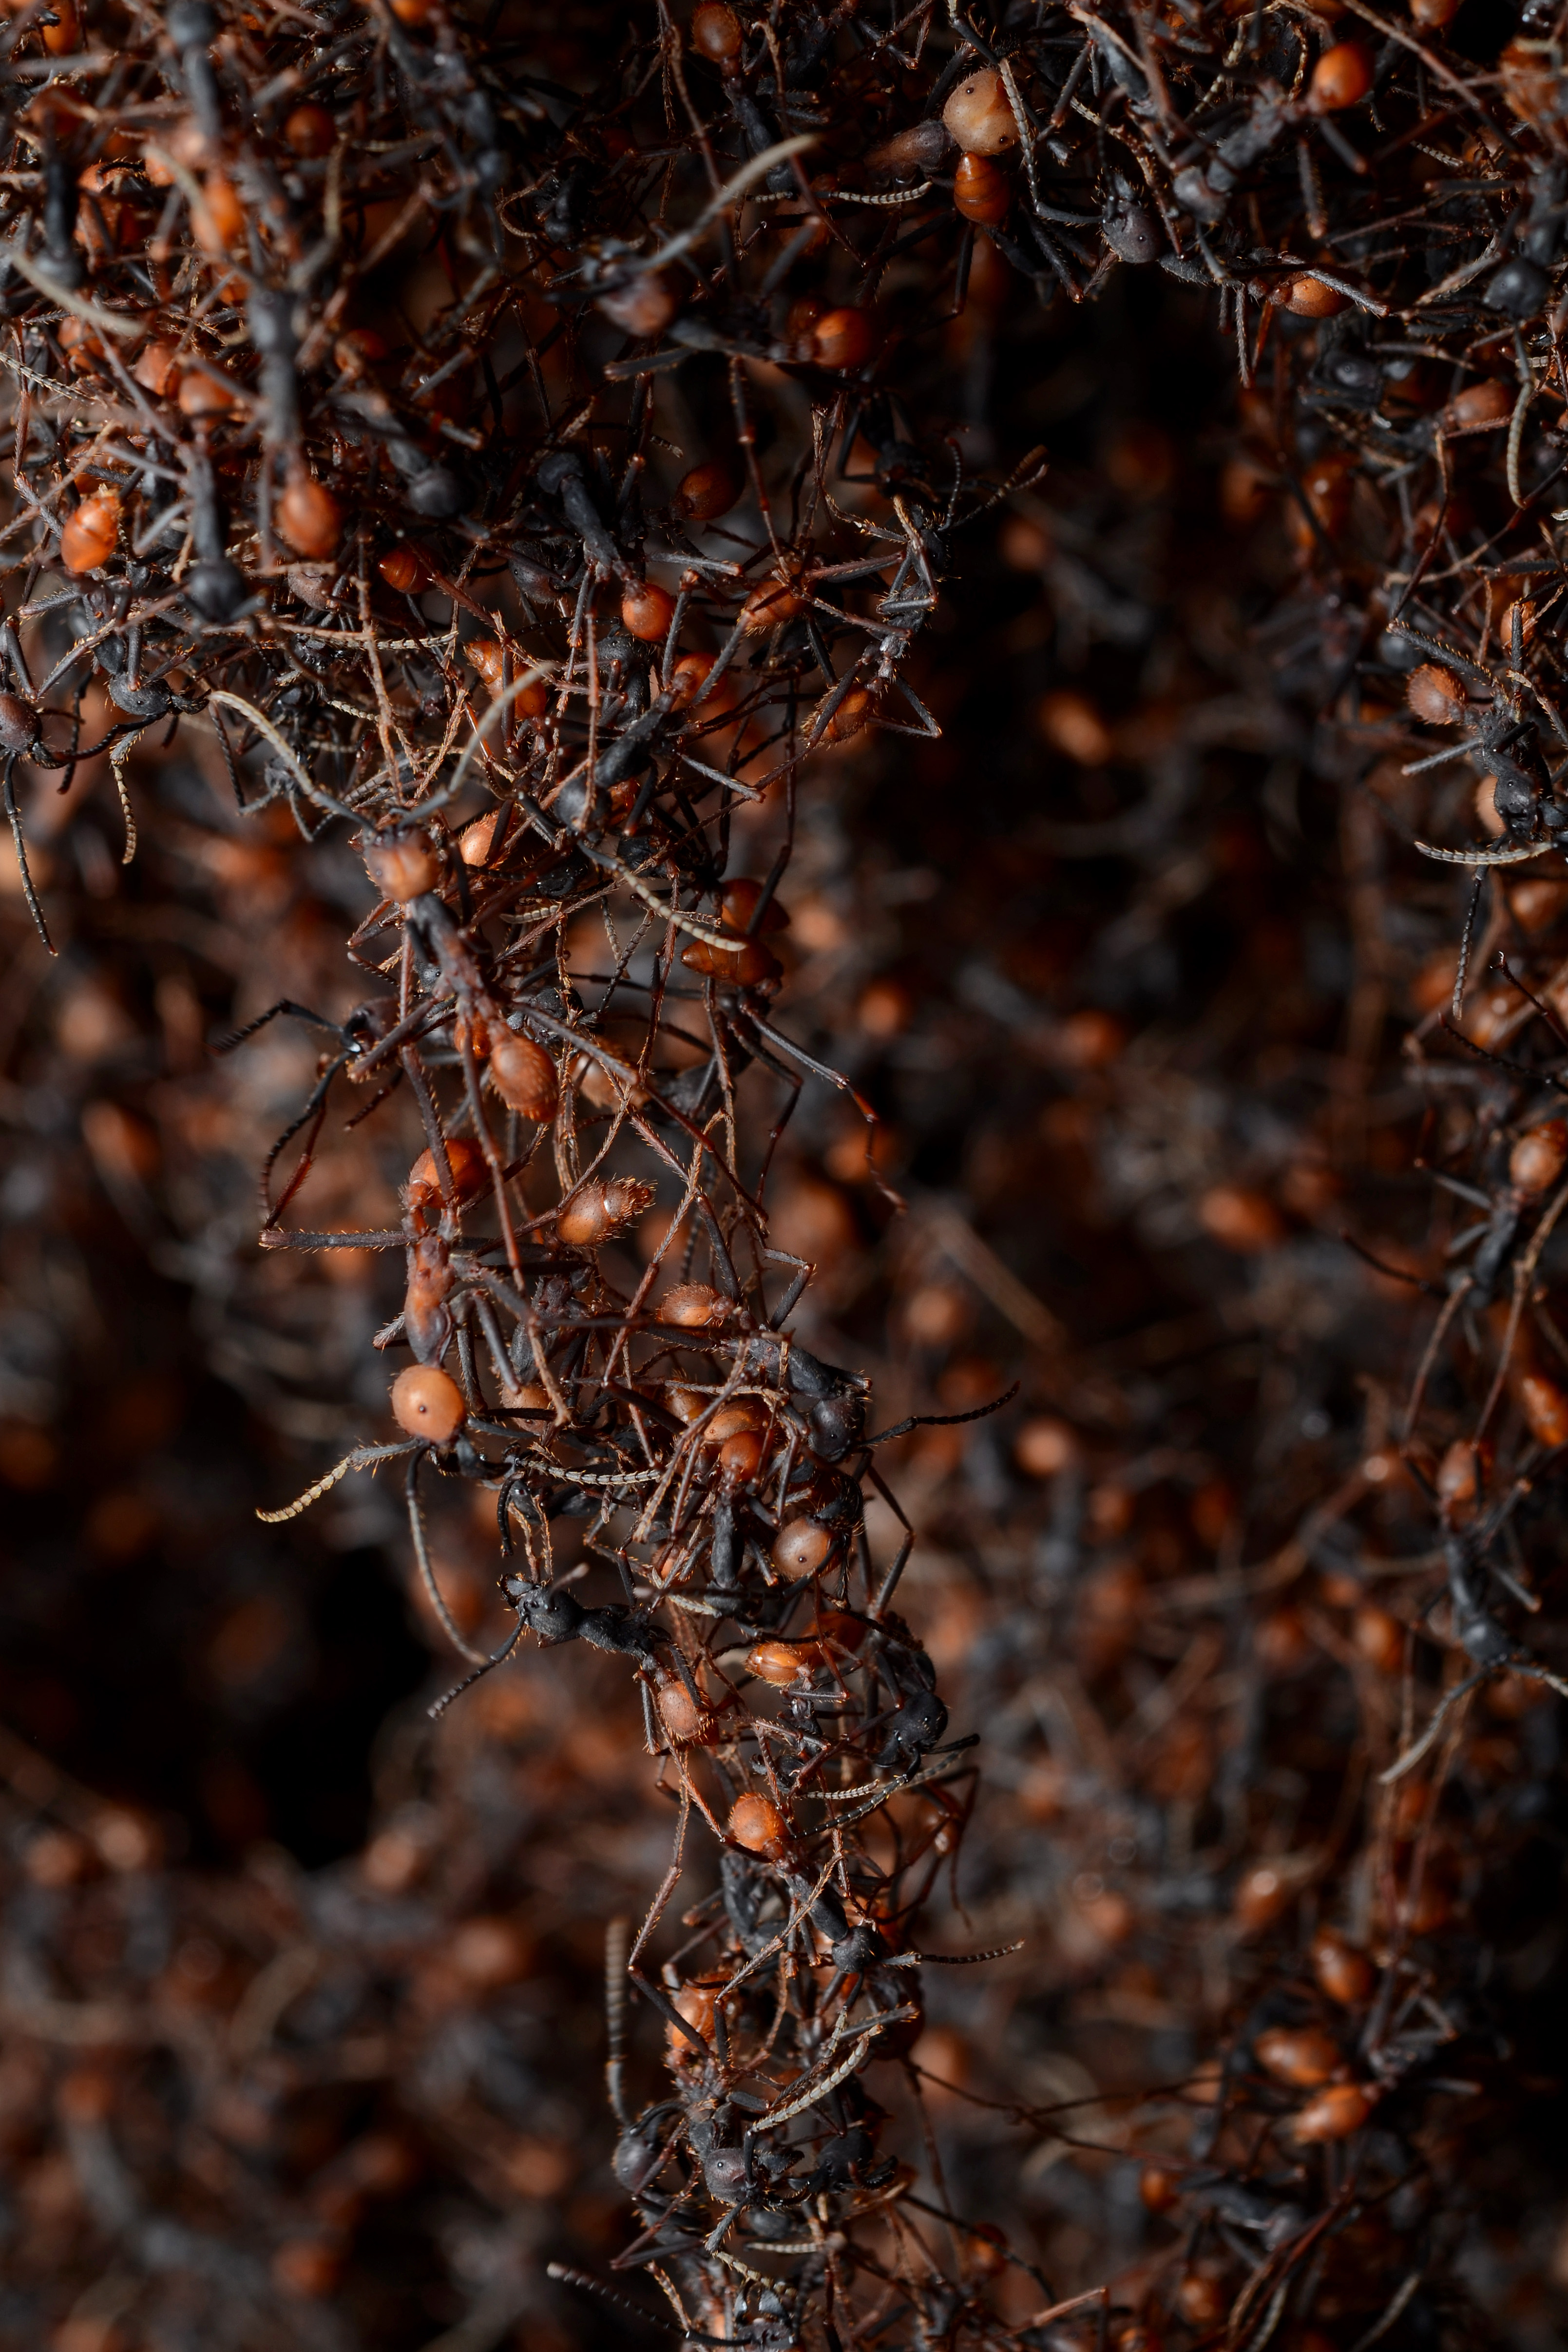
\includegraphics[angle=270, width=\textwidth]{ant_bridge}
\end{column}
\end{columns}
\vspace{1ex}
\begin{columns}
\begin{column}{0.05\textwidth}
\end{column}
\begin{column}{0.27\textwidth}
\centering
cell {\tiny\cite{clare_and_ben_2017}}
\end{column}
\begin{column}{0.07\textwidth}
\end{column}
\begin{column}{0.27\textwidth}
\centering
ant {\tiny\cite{quinzani_2008}}
\end{column}
\begin{column}{0.07\textwidth}
\end{column}
\begin{column}{0.27\textwidth}
\centering
ant colony {\tiny\cite{gallice_2011}}
\end{column}
\end{columns}
\vspace{2ex}
\caption{Analogy between (\subref{fig:natural}) natural and (\subref{fig:simulated}) simulated hierarchical fraternal transitions of individuality.}

\end{figure}


\end{frame}

\begin{frame}{What is an Individual?}

commonly-cited characteristics:
\begin{itemize}
\item close coordination and cooperation
\item reproductive division of labor
\item reproductive bottlenecks
\item loss of ability to replicate independently
\item \cite{ereshefsky2015rethinking, bouchard2013symbiotic}.
\end{itemize}

\end{frame}

\begin{frame}{Mission Statement}
Want to study fraternal transitions in individuality?

\pause
\vspace{2ex}

Need a model where such transitions to occur
\begin{itemize}
\item reliably
\item detectably
\end{itemize}

\pause
\vspace{2ex}

Our model: DISHTINY \footnotesize{(DIStributed Hierarchical Transitions in IndividualitY)}

\end{frame}
